%! Author = Ian
%! Date = 12/4/2023

% Preamble
\documentclass[11pt]{article}

% Packages
\usepackage{amsmath}
\usepackage{graphics}
\usepackage{graphicx}

\title{Assignment 5 Writeup}
\author{Ian Chen}
\date{\today}

% Document
\begin{document}
    \maketitle


    \section{Face Detection}

    \begin{itemize}
        \item \textit{Face Classification}\newline
        I used the Viola-Jones algorithm, which uses AdaBoosting to train a strong classifier from a
        subset of Haar-like features. The algorithm is able to achieve a high detection rate while
        minimizing the number of false positives. I generated faces using the FDDB dataset with
        their included bounding boxes.\newline
        I scaled the faces to 24x24 pixels, and the areas of the image not covered by the face were
        deemed non-face regions. I generated the integral images of the training set and its
        corresponding haar-like features. I then used a subset of these features to train the
        boosting algorithm.\newline
        Top classifiers: Decision Stump: (parity=-1, feature\_index=307, threshold=1212
        .2045312499986, error=0.2754251247073025, alpha=-0.96726929195333)\newline
        Decision Stump: (parity=-1, feature\_index=701, threshold=87.74951562500792, error=0
        .29285768037256815, alpha=-0.8815451878903284)\newline
        Decision Stump: (parity=1, feature\_index=402, threshold=-175.16371425779653, error=0
        .3254346857998712, alpha=-0.728906721017052)\newline
        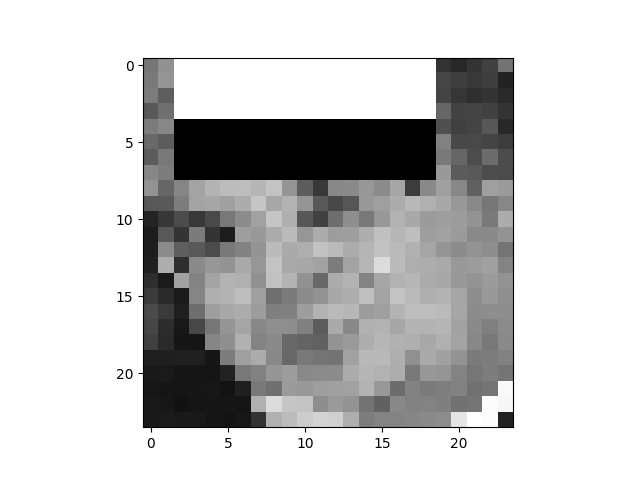
\includegraphics[width=0.3\textwidth]{Output Pictures/rec_1}
        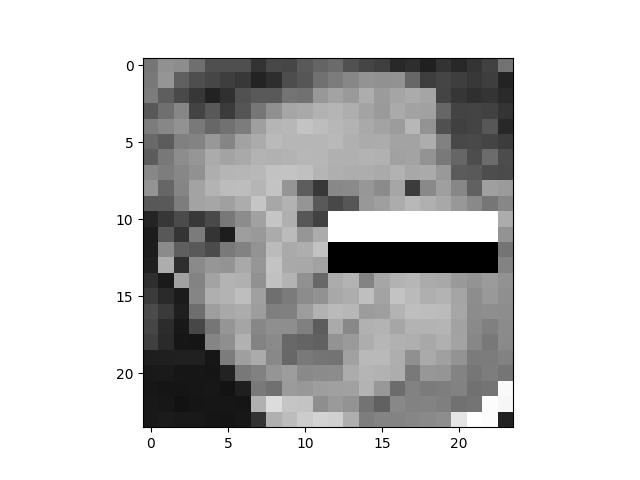
\includegraphics[width=0.3\textwidth]{Output Pictures/rec_2}
        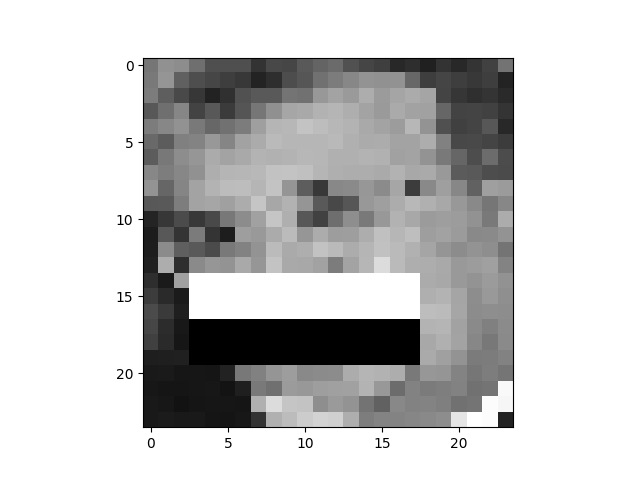
\includegraphics[width=0.3\textwidth]{Output Pictures/rec_3}

        \item \textit{Sliding Window + Human Classification}\newline
        I used the Viola-Jones algorithm along with the classifier cascade. The algorithm is also
        able to run in real time, as I used the classifier cascade to quickly reject non-face
        regions.\newline
        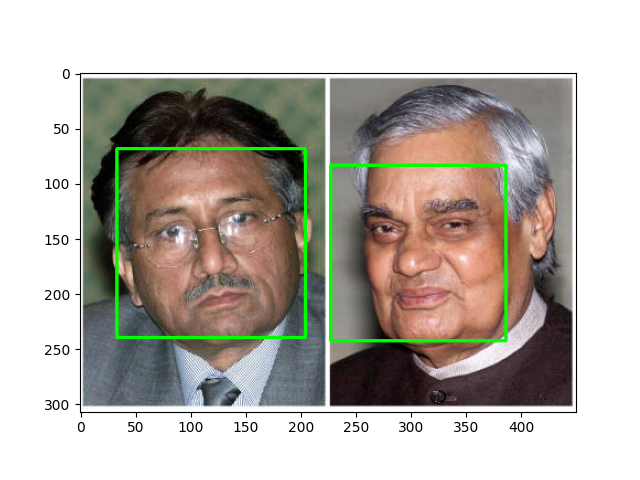
\includegraphics[width=0.3\textwidth]{Output Pictures/ex_1}
        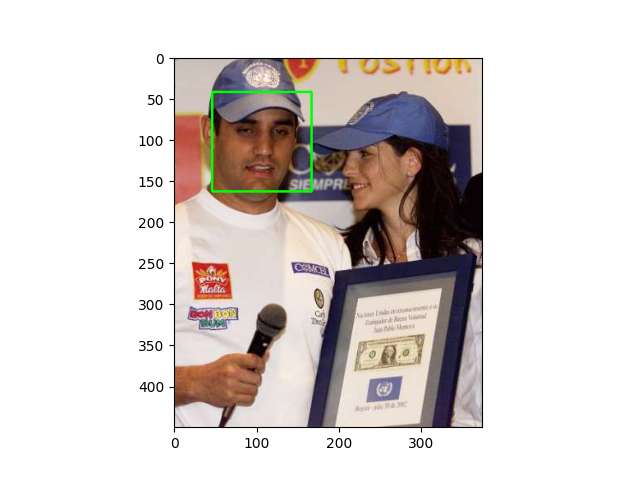
\includegraphics[width=0.3\textwidth]{Output Pictures/ex_2}
        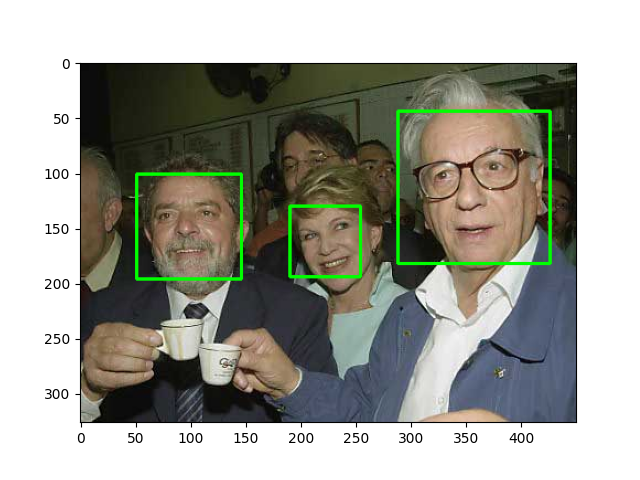
\includegraphics[width=0.3\textwidth]{Output Pictures/ex_3}
        The algorithm is able to detect faces in the images, but with the classifier cascade, it
        needs fine-tuning to reduce the number of false positives while maintaining a high detection
        rate.\newline
        % TODO: Answer

    \end{itemize}


    \section{Extra Credit}

    \begin{itemize}
        \item \textit{Object Detection}
        % TODO: Answer

        \item \textit{Running Time}
        % TODO: Answer

        \item \textit{Creative Ideas}
        % TODO: Answer

    \end{itemize}
\end{document}